%%%%%%%%%%%%%%%%%%%%%%%%%%%%%%%%%%%%%%%%%
% Beamer Presentation
% LaTeX Template
% Version 1.0 (10/11/12)
%
% This template has been downloaded from:
% http://www.LaTeXTemplates.com
%
% License:
% CC BY-NC-SA 3.0 (http://creativecommons.org/licenses/by-nc-sa/3.0/)
%
%%%%%%%%%%%%%%%%%%%%%%%%%%%%%%%%%%%%%%%%%

%----------------------------------------------------------------------------------------
%	PACKAGES AND THEMES
%----------------------------------------------------------------------------------------

\documentclass{beamer}

\mode<presentation> {

% The Beamer class comes with a number of default slide themes
% which change the colors and layouts of slides. Below this is a list
% of all the themes, uncomment each in turn to see what they look like.

%\usetheme{default}
%\usetheme{AnnArbor}
%\usetheme{Antibes}
%\usetheme{Bergen}
%\usetheme{Berkeley}
%\usetheme{Berlin}
%\usetheme{Boadilla}
%\usetheme{CambridgeUS}
%\usetheme{Copenhagen}
%\usetheme{Darmstadt}
%\usetheme{Dresden}
%\usetheme{Frankfurt}
%\usetheme{Goettingen}
%\usetheme{Hannover}
%\usetheme{Ilmenau}
%\usetheme{JuanLesPins}
%\usetheme{Luebeck}
\usetheme{Madrid}
%\usetheme{Malmoe}
%\usetheme{Marburg}
%\usetheme{Montpellier}
%\usetheme{PaloAlto}
%\usetheme{Pittsburgh}
%\usetheme{Rochester}
%\usetheme{Singapore}
%\usetheme{Szeged}
%\usetheme{Warsaw}

% As well as themes, the Beamer class has a number of color themes
% for any slide theme. Uncomment each of these in turn to see how it
% changes the colors of your current slide theme.

%\usecolortheme{albatross}
%\usecolortheme{beaver}
%\usecolortheme{beetle}
%\usecolortheme{crane}
%\usecolortheme{dolphin}
%\usecolortheme{dove}
%\usecolortheme{fly}
%\usecolortheme{lily}
%\usecolortheme{orchid}
%\usecolortheme{rose}
%\usecolortheme{seagull}
%\usecolortheme{seahorse}
%\usecolortheme{whale}
%\usecolortheme{wolverine}

%\setbeamertemplate{footline} % To remove the footer line in all slides uncomment this line
%\setbeamertemplate{footline}[page number] % To replace the footer line in all slides with a simple slide count uncomment this line

%\setbeamertemplate{navigation symbols}{} % To remove the navigation symbols from the bottom of all slides uncomment this line
}

\usepackage{graphicx} % Allows including images
\usepackage{grffile}
\usepackage{booktabs} % Allows the use of \toprule, \midrule and \bottomrule in tables
\usepackage{caption}
\usepackage{subcaption}
\usepackage{lmodern}
\usepackage{siunitx}
\sisetup{separate-uncertainty=true}

\graphicspath{{figures/}}

%----------------------------------------------------------------------------------------
%	TITLE PAGE
%----------------------------------------------------------------------------------------

\title[High Energy Analysis]{High Energy Analysis and Application to Dark Matter
Search} % The short title appears at the bottom of every slide, the full title is only on the title page

\author{Michinari Sakai} % Your name
\institute[UH] % Your institution as it will appear on the bottom of every slide, may be shorthand to save space
{
University of Hawaii, Manoa \\ % Your institution for the title page
\medskip
\textit{michinar@hawaii.edu} % Your email address
}
\date{\today} % Date, can be changed to a custom date

\begin{document}

\begin{frame}
\titlepage % Print the title page as the first slide
\end{frame}

\begin{frame}
\frametitle{Overview} % Table of contents slide, comment this block out to remove it
\tableofcontents % Throughout your presentation, if you choose to use \section{} and \subsection{} commands, these will automatically be printed on this slide as an overview of your presentation
\end{frame}

%----------------------------------------------------------------------------------------
%	PRESENTATION SLIDES
%----------------------------------------------------------------------------------------

%------------------------------------------------
%\section{First Section} % Sections can be created in order to organize your presentation into discrete blocks, all sections and subsections are automatically printed in the table of contents as an overview of the talk
%------------------------------------------------

%\subsection{Subsection Example} % A subsection can be created just before a set of slides with a common theme to further break down your presentation into chunks

\section{Previous work}
\begin{frame}[t]{Previously at UCLA I talked about...}
	\begin{itemize}
		\item Energy callibration @ high energies using minimum-ionizing cosmic
			ray $\mu$
		\item Explored ways to cut PMT prepulsing\\
			$\implies$ conclusion: difficult\\
			$\implies$ useful to keep all gain channel signals\\
			$\implies$ but prepulsing is $\sim$few$\%$ effect so $\nu$
			directionality fitter tuned to be insensitive to prepulsing
		\item $\nu$ directionality fitter tested using MC\\
			$\implies$ fitter valid for energy $> \sim\SI{500}{MeV}$
	\end{itemize}
\end{frame}

\section{Signal and background scheme}
\begin{frame}
	\frametitle{Signal: WIMP annihilation induced $\nu$}
	\begin{figure}
		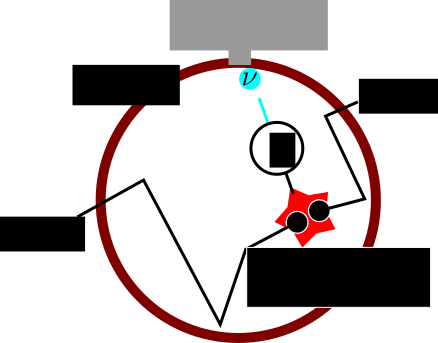
\includegraphics[width=0.6\linewidth]{detection_scheme.pdf}
	\end{figure}
\end{frame}

\begin{frame}
	\frametitle{Background: Atmospheric $\nu$}
	\centering
	\begin{figure}
		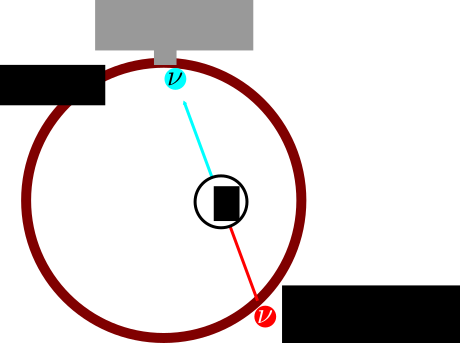
\includegraphics[width=0.6\linewidth]{background_model.pdf}
	\end{figure}
\end{frame}

\section{Model building}
\subsection{Earth model and neutrino oscillation w/ matter effects}
\begin{frame}
	\frametitle{Earth Model (PREM)}
	\begin{figure}
		\centering
		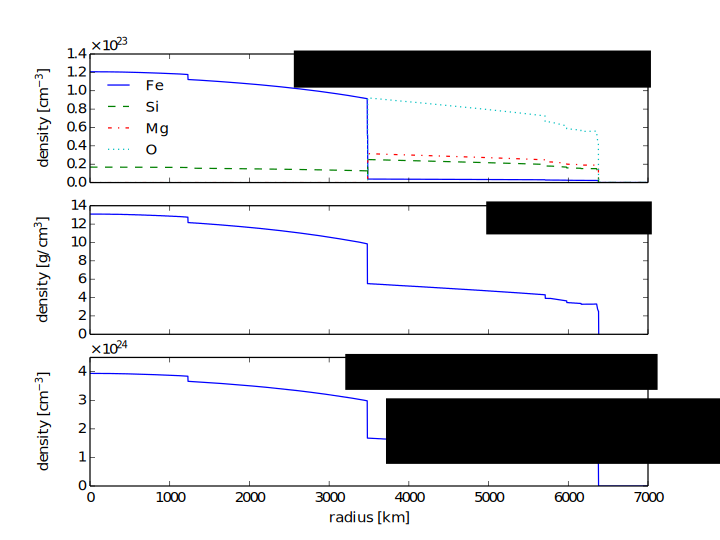
\includegraphics[width=0.75\linewidth]{earth_density.pdf}
	\end{figure}
\end{frame}

\begin{frame}
	\frametitle{Neutrino Oscillation Parameters (PDG 2014)}
	\begin{itemize}
		\item $\sin^2{(2\theta_{12})} =
			\num{0.846\pm0.021}
			\rightarrow \theta_{12} = \SI{33.45}{\degree}$
		\item $\sin^2{(2\theta_{13})} =
			\num{9.3\pm0.8e-2}
			\rightarrow \theta_{13} = \SI{8.88}{\degree}$
		\item $\sin^2{(2\theta_{23})} = 0.999^{+0.001}_{-0.018}
			\rightarrow \theta_{23} = \SI{44.09}{\degree}$ (normal hierarchy)
		\item $\Delta m_{21}^2 = \SI{7.53\pm0.18e-5}{\electronvolt\square}$
		\item $\Delta m_{31}^2 = \SI{2.52\pm0.06e-3}{\electronvolt\square}$
			(normal hierarchy)
	\end{itemize}
\end{frame}

\begin{frame}
	\frametitle{$\nu$ produced in Earth or atmosphere will oscillate by the time
	it reaches KamLAND}
	\begin{figure}
		\centering
			\includegraphics[width=0.85\linewidth]{nu_oscillation_in_earth.pdf}
	\end{figure}
\end{frame}

\begin{frame}
	\frametitle{$\nu$ oscillation probability at \SI{1}{GeV}}
	KamLAND is at radius $= \SI{6378}{\kilo\meter}$ and angle $=
	\SI{0}{\degree}$.

	Following is cross-section of Earth through Earth center and KamLAND.

	Color represents oscillation probability $P(\nu_{\alpha} \rightarrow
	\nu_{\beta})$ for $\nu_{\alpha}$ created in Earth and $\nu_{\beta}$ arriving
	at KamLAND.
	\begin{figure}
		\centering
		\begin{subfigure}[b]{0.49\linewidth}
			\caption{ $\nu_{e} \rightarrow \nu_{e}$ }
			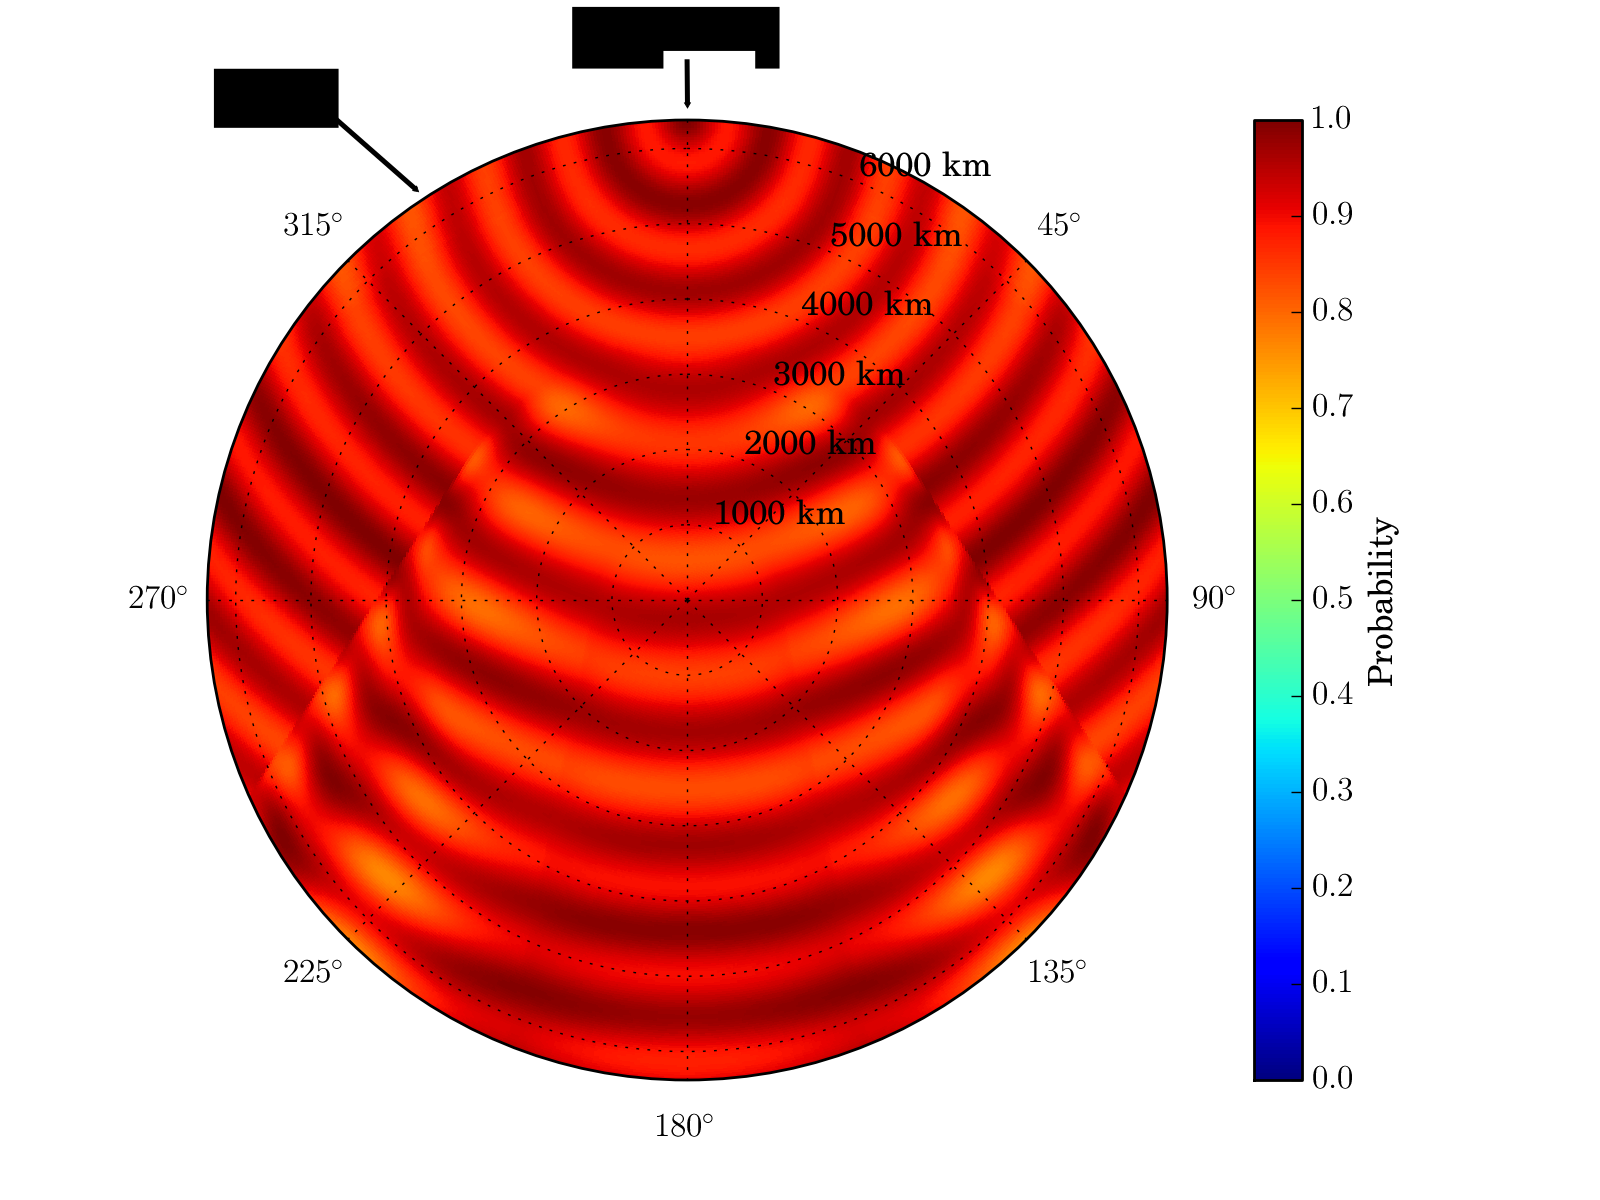
\includegraphics[width=\linewidth]{earth_1.0gev_nue2nue_throughEarth.png}
		\end{subfigure}
		\begin{subfigure}[b]{0.49\linewidth}
			\caption{ $\nu_{e} \rightarrow \nu_{\mu}$ }
			\includegraphics[width=\linewidth]{earth_1.0gev_nue2numu_throughEarth.png}
		\end{subfigure}
	\end{figure}
\end{frame}

\begin{frame}
	\frametitle{$\nu$ oscillation probability at \SI{10}{GeV}}
	KamLAND is at radius $= \SI{6378}{\kilo\meter}$ and angle $=
	\SI{0}{\degree}$.

	Following is cross-section of Earth through Earth center and KamLAND.

	Color represents oscillation probability $P(\nu_{\alpha} \rightarrow
	\nu_{\beta})$ for $\nu_{\alpha}$ created in Earth and $\nu_{\beta}$ arriving
	at KamLAND.
	\begin{figure}
		\centering
		\begin{subfigure}[b]{0.49\linewidth}
			\caption{ $\nu_{e} \rightarrow \nu_{e}$ }
			\includegraphics[width=\linewidth]{earth_10.0gev_nue2nue_throughEarth.png}
		\end{subfigure}
		\begin{subfigure}[b]{0.49\linewidth}
			\caption{ $\nu_{e} \rightarrow \nu_{\mu}$ }
			\includegraphics[width=\linewidth]{earth_10.0gev_nue2numu_throughEarth.png}
		\end{subfigure}
	\end{figure}
\end{frame}

\begin{frame}
	\frametitle{Oscillation Probability for Atmospheric $\nu$ Background}
	\begin{figure}
		\begin{subfigure}[]{0.45\linewidth}
			\centering
			\vspace{-15pt}
			\caption{ $\nu_{e} \rightarrow \nu_{e}$ }
			\vspace{-8pt}
			\includegraphics[width=\linewidth]{atm_nue2nue.pdf} \\
			\vspace{-10pt}
			\caption*{(averaged to Honda bins)}
			\vspace{-8pt}
			\includegraphics[width=\linewidth]{atm_nue2nue_avg.pdf}
			\vspace{-13pt}
		\end{subfigure}
		\begin{subfigure}[]{0.45\linewidth}
			\centering
			\vspace{-15pt}
			\caption{ $\nu_{e} \rightarrow \nu_{\mu}$ }
			\vspace{-8pt}
			\includegraphics[width=\linewidth]{atm_nue2numu.pdf} \\
			\vspace{-10pt}
			\caption*{(averaged to Honda bins)}
			\vspace{-8pt}
			\includegraphics[width=\linewidth]{atm_nue2numu_avg.pdf}
			\vspace{-13pt}
		\end{subfigure}
	\end{figure}
\end{frame}

\begin{frame}
	\frametitle{Oscillation Probability for Atmospheric $\nu$ Background}
	\begin{figure}
		\begin{subfigure}[]{0.45\linewidth}
			\centering
			\vspace{-15pt}
			\caption{ $\nu_{\mu} \rightarrow \nu_{e}$ }
			\vspace{-8pt}
			\includegraphics[width=\linewidth]{atm_numu2nue.pdf} \\
			\vspace{-10pt}
			\caption*{(averaged to Honda bins)}
			\vspace{-8pt}
			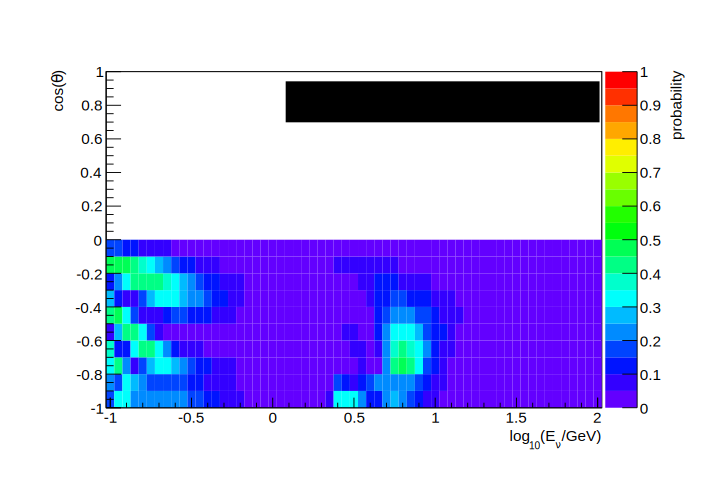
\includegraphics[width=\linewidth]{atm_numu2nue_avg.pdf}
		\end{subfigure}
		\begin{subfigure}[]{0.45\linewidth}
			\centering
			\vspace{-15pt}
			\caption{ $\nu_{\mu} \rightarrow \nu_{\mu}$ }
			\vspace{-8pt}
			\includegraphics[width=\linewidth]{atm_numu2numu.pdf} \\
			\vspace{-10pt}
			\caption*{(averaged to Honda bins)}
			\vspace{-8pt}
			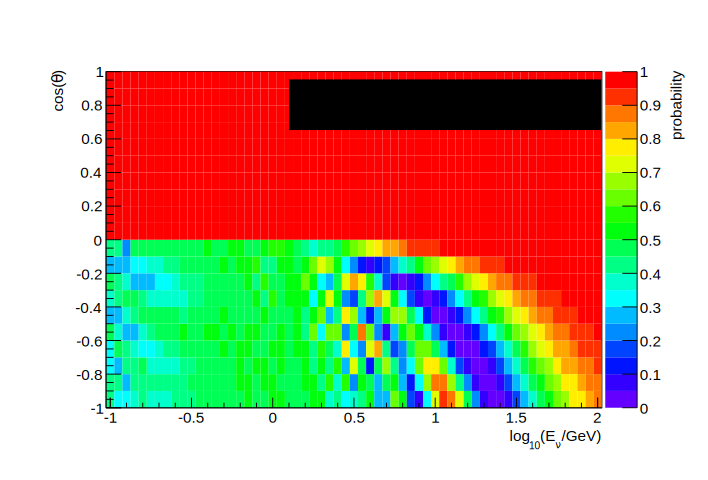
\includegraphics[width=\linewidth]{atm_numu2numu_avg.pdf}
		\end{subfigure}
	\end{figure}
\end{frame}

\subsection{Background model (M. Honda tables)}
\begin{frame}
	\frametitle{Atmospheric $\nu_{e}$ Background}
	\begin{figure}
		\centering
		\begin{subfigure}[b]{0.49\linewidth}
			\caption*{ w/o oscillation }
			\includegraphics[width=\linewidth]{atm_nue_hist.pdf}
		\end{subfigure}
		\begin{subfigure}[b]{0.49\linewidth}
			\caption*{ w/ oscillation }
			\includegraphics[width=\linewidth]{atm_nue_osc_hist.pdf}
		\end{subfigure}
	\end{figure}
\end{frame}

\begin{frame}
	\frametitle{Atmospheric $\nu_{\mu}$ Background}
	\begin{figure}
		\centering
		\begin{subfigure}[b]{0.49\linewidth}
			\caption*{ w/o oscillation }
			\includegraphics[width=\linewidth]{atm_numu_hist.pdf}
		\end{subfigure}
		\begin{subfigure}[b]{0.49\linewidth}
			\caption*{ w/ oscillation }
			\includegraphics[width=\linewidth]{atm_numu_osc_hist.pdf}
		\end{subfigure}
	\end{figure}
\end{frame}

\subsection{Dark matter capture simulation (DarkSUSY)}
\begin{frame}
	\frametitle{Dark Matter Capture in Earth}
	Spin-independent cross-section $\sigma_{\mathrm{SI}} =
	\SI{1e-40}{\square\centi\meter}$
	\begin{figure}
		\centering
		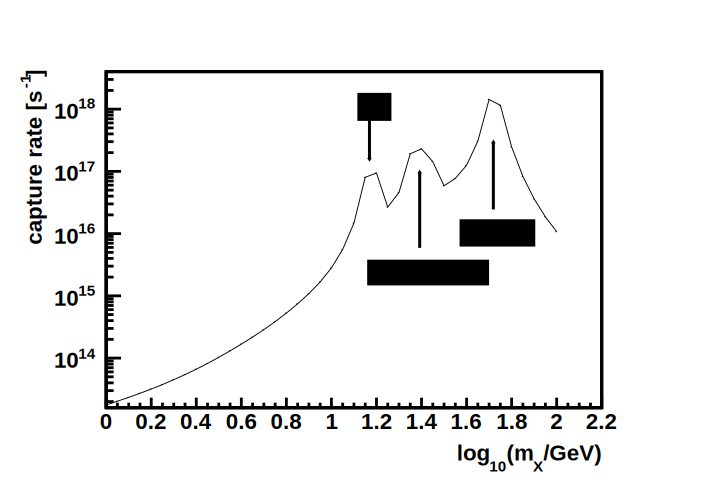
\includegraphics[width=0.75\linewidth]{wimp_capture_rate.pdf}
	\end{figure}
\end{frame}

\subsection{Signal model (WimpSim)}
\begin{frame}
	\frametitle{Signal from $m_X = \SI{10}{\giga\electronvolt}$,
		$\chi \overline{\chi} \rightarrow \nu_{e} \overline{\nu_{e}}$}
	(Generated from \num{e7} $\chi \overline{\chi}$ annihilations)
	\begin{figure}
		\centering
		\begin{subfigure}[b]{0.49\linewidth}
			\caption*{ $\nu_{e}$ flux }
			\includegraphics[width=\linewidth]{hist_flux_nue_from_10gev_mx_to_nuenuebar.pdf}
		\end{subfigure}
		\begin{subfigure}[b]{0.49\linewidth}
			\caption*{ $\overline{\nu}_{e}$ flux }
			\includegraphics[width=\linewidth]{hist_flux_nuebar_from_10gev_mx_to_nuenuebar.pdf}
		\end{subfigure}
	\end{figure}
\end{frame}

\begin{frame}
	\frametitle{Signal from $m_X = \SI{10}{\giga\electronvolt}$,
		$\chi \overline{\chi} \rightarrow \tau \overline{\tau}$}
	(Generated from \num{e7} $\chi \overline{\chi}$ annihilations)
	\begin{figure}
		\centering
		\begin{subfigure}[b]{0.49\linewidth}
			\caption*{ $\nu_{e}$ flux }
			\includegraphics[width=\linewidth]{hist_flux_nue_from_10gev_mx_to_tautaubar.pdf}
		\end{subfigure}
		\begin{subfigure}[b]{0.49\linewidth}
			\caption*{ $\overline{\nu}_{e}$ flux }
			\includegraphics[width=\linewidth]{hist_flux_nuebar_from_10gev_mx_to_tautaubar.pdf}
		\end{subfigure}
	\end{figure}
\end{frame}

\begin{frame}
	\frametitle{Signal from $m_X = \SI{10}{\giga\electronvolt}$,
		$\chi \overline{\chi} \rightarrow b \overline{b}$}
	(Generated from \num{e7} $\chi \overline{\chi}$ annihilations)
	\begin{figure}
		\centering
		\begin{subfigure}[b]{0.49\linewidth}
			\caption*{ $\nu_{e}$ flux }
			\includegraphics[width=\linewidth]{hist_flux_nue_from_10gev_mx_to_bbbar.pdf}
		\end{subfigure}
		\begin{subfigure}[b]{0.49\linewidth}
			\caption*{ $\overline{\nu}_{e}$ flux }
			\includegraphics[width=\linewidth]{hist_flux_nuebar_from_10gev_mx_to_bbbar.pdf}
		\end{subfigure}
	\end{figure}
\end{frame}

\section{Data}
\subsection{Data selection}
\begin{frame}
	\frametitle{Data Selection}
	\begin{itemize}
		%\item Date: ~
		\item Runs: \numrange{1330}{12475}
		\item Total Live Time: 3671 days
		\item Selection Criteria: $\mathrm{nHit}_{\mathrm{OD}} < 5$,
			$E_{\mathrm{Kat}} >= \SI{1}{GeV}$
	\end{itemize}
\end{frame}

\begin{frame}
	\frametitle{Reconstructed Vertex}
	\begin{figure}
		\centering
		\begin{subfigure}[b]{0.49\linewidth}
			\caption*{ Reconstructed energy $> \SI{30}{MeV}$ }
			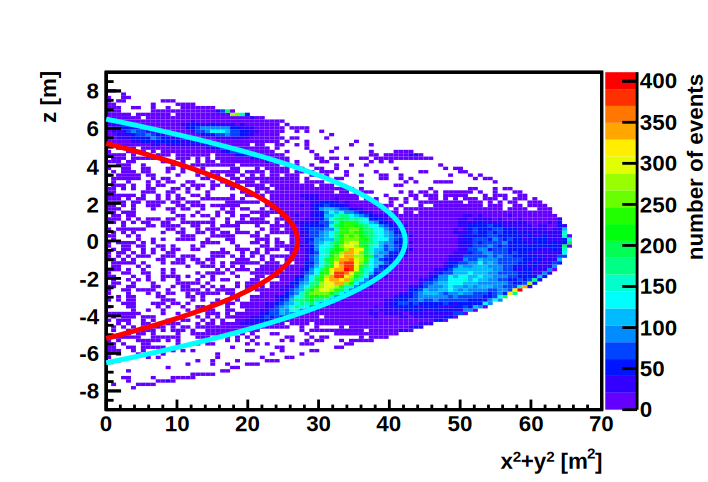
\includegraphics[width=\linewidth]{kat_vertex_min30mev.pdf}
		\end{subfigure}
		\begin{subfigure}[b]{0.49\linewidth}
			\caption*{ Reconstructed energy $> \SI{1}{GeV}$ }
			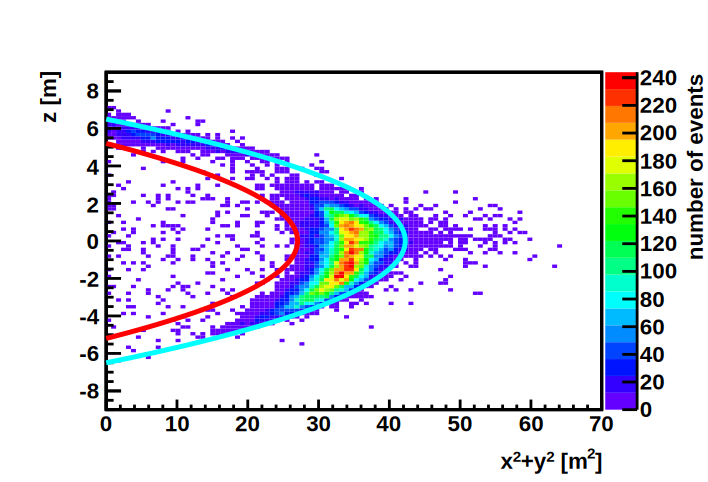
\includegraphics[width=\linewidth]{kat_vertex_min1gev.pdf}
		\end{subfigure} \\
		\begin{itemize}
			\item Black line: \SI{6.5}{\meter} radius balloon
			\item Red line: \SI{5.2}{\meter} radius fiducial volume
			\item T2K veto applied by Shimizu-san
		\end{itemize}
	\end{figure}
\end{frame}

\subsection{Fit Model and Data}
\begin{frame}
	\frametitle{Fit data to background model}
	\begin{figure}
		\centering
		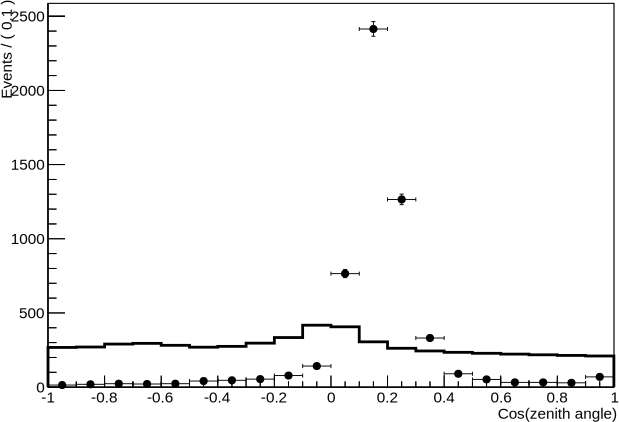
\includegraphics[width=0.85\linewidth]{fit_data_to_bkg_model_noChi2TCut.pdf}
	\end{figure}
\end{frame}

\begin{frame}
	\frametitle{$\chi^{2}$ of data/model fit vs $\chi^{2}_{\mathrm{time}}$ cut}
	\begin{figure}
		\centering
		\includegraphics[width=0.8\linewidth]{chi2tcut_vs_fitGoodness.pdf}

		At $\SI{90}{\percent}$ confidence level $\chi^{2}_{\mathrm{T}}$ cut
		$= 3.32$
	\end{figure}
\end{frame}

\begin{frame}
	\frametitle{Vertex $\chi^{2}_{\mathrm{time}}$ (test of event point-likeness)}
	\begin{figure}
		\centering
		\begin{figure}
			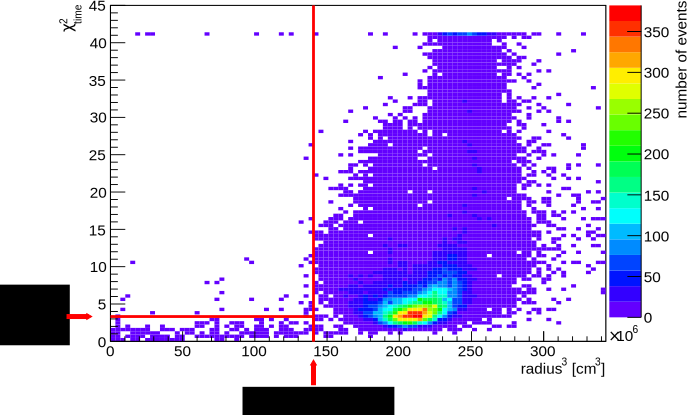
\includegraphics[width=0.9\linewidth]{chi2t_vs_radius.pdf}
		\end{figure}
	\end{figure}
\end{frame}

\begin{frame}
	\frametitle{Fit data to background model (with $\chi^{2}_{T}$ cut)}
	\begin{figure}
		\centering
		\begin{subfigure}[b]{0.49\linewidth}
			\caption*{No $\chi^{2}_{T}$ cut}
			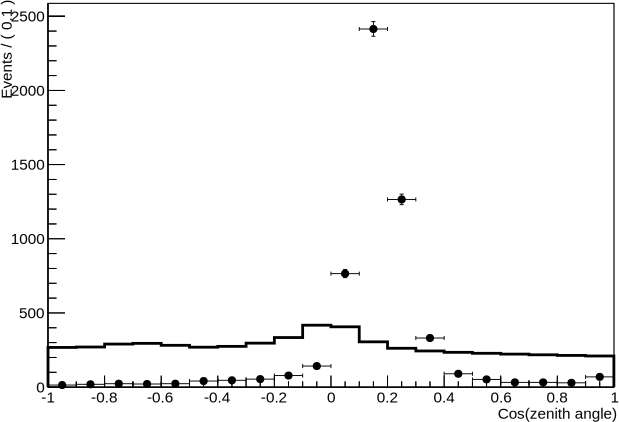
\includegraphics[width=\linewidth]{fit_data_to_bkg_model_noChi2TCut.pdf}
		\end{subfigure}
		\begin{subfigure}[b]{0.49\linewidth}
			\caption*{$\chi^{2}_{T}$ cut $= 3.32$}
			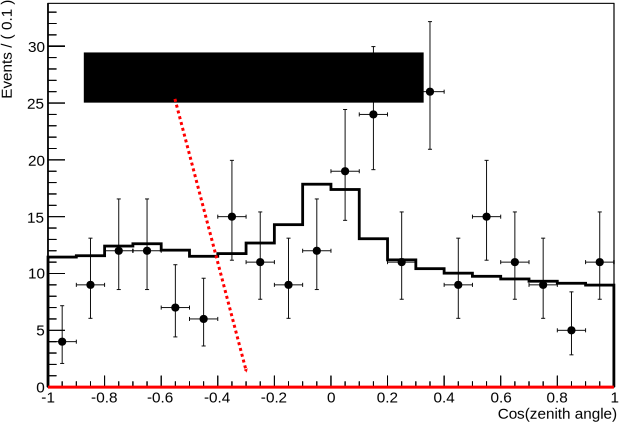
\includegraphics[width=\linewidth]{fit_data_to_bkg_model_3_32Chi2TCut.pdf}
		\end{subfigure}
		
	\end{figure}
\end{frame}

\begin{frame}[t]{Event rate equation}
	\begin{equation*}
		\mathrm{rate}_{\mathrm{signal}} = \Gamma_{\mathrm{A}} \times
		\sum\limits_{\substack{\mathrm{channel} = i\\ \nu-\mathrm{flavor}= \alpha}}
		\left[
			B_{i} \int dE_{\alpha} \frac{dN_{i,\alpha}}{dE_{\alpha}}
			\frac{\sigma_{\mathrm{effective}}(E_{\alpha})}
			{4\pi R_{\mathrm{Earth}}^2}
		\right]
	\end{equation*}
	\begin{itemize}
		\item $\Gamma_{A} = \frac{1}{2}\Gamma_{C}$ ($\chi \overline{\chi}$
			annihilation rate at equilibrium)
		\item $\Gamma_{C} = \sigma_{\chi-\mathrm{nucleon}} C_{0}$ ($\chi$ capture rate)
		\item $E_{\alpha}$ (energy of neutrino for flavor $\alpha$)
		\item $N_{i,\alpha}$ (neutrino yield of flavor $\alpha$ per
			annihilation for channel $i$)
		\item $\sigma_{\mathrm{effective},\alpha}(E_{\alpha})$ (effective
			detector cross-section)
		\item $R_{\mathrm{Earth}}$ (radius of Earth)
	\end{itemize}
	$\therefore$ \SI{90}{\percent} C.L. bound on $\mathrm{rate}_{\mathrm{signal}}$
	$\implies$ \SI{90}{\percent} C.L. bound on $\sigma_{\chi-\mathrm{nucleon}}$
\end{frame}

\subsection{Dark matter bounds}
\begin{frame}
	\frametitle{WIMP $\sigma_{\mathrm{SI}}$ bounds (\SI{90}{\percent} C.L.)}
	\begin{figure}
		\centering
		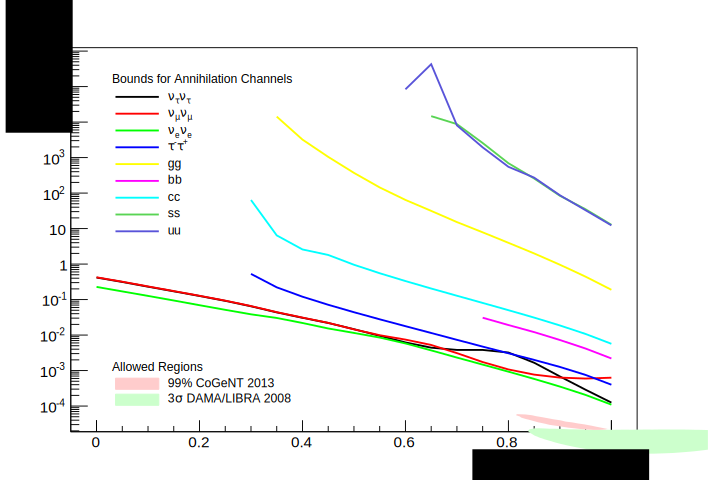
\includegraphics[width=0.85\linewidth]{dmXSec_vs_log10mx.pdf}
	\end{figure}
\end{frame}

\begin{frame}
	\frametitle{To do}
	\begin{itemize}
		\item KLG4 high energy simulation taking a long time (now $\sim$half
			done, $\sim$4 months more using $\sim$100 cores) \\
			$\implies$ need to discuss with simulation expert to optimize KLG4
			for large amount of photons or continue running as is
		\item OD inefficiency for $\mu$-veto \\
			$\implies$ maybe need to simulated $\mu$ background and fit to data
			instead of finding a $\chi_{T}^{2}$ cut to reduce $\mu$ background
	\end{itemize}
\end{frame}

%\begin{frame}
%\frametitle{Paragraphs of Text}
%Sed iaculis dapibus gravida. Morbi sed tortor erat, nec interdum arcu. Sed id lorem lectus. Quisque viverra augue id sem ornare non aliquam nibh tristique. Aenean in ligula nisl. Nulla sed tellus ipsum. Donec vestibulum ligula non lorem vulputate fermentum accumsan neque mollis.\\~\\
%
%Sed diam enim, sagittis nec condimentum sit amet, ullamcorper sit amet libero. Aliquam vel dui orci, a porta odio. Nullam id suscipit ipsum. Aenean lobortis commodo sem, ut commodo leo gravida vitae. Pellentesque vehicula ante iaculis arcu pretium rutrum eget sit amet purus. Integer ornare nulla quis neque ultrices lobortis. Vestibulum ultrices tincidunt libero, quis commodo erat ullamcorper id.
%\end{frame}
%
%%------------------------------------------------
%
%\begin{frame}
%\frametitle{Bullet Points}
%\begin{itemize}
%\item Lorem ipsum dolor sit amet, consectetur adipiscing elit
%\item Aliquam blandit faucibus nisi, sit amet dapibus enim tempus eu
%\item Nulla commodo, erat quis gravida posuere, elit lacus lobortis est, quis porttitor odio mauris at libero
%\item Nam cursus est eget velit posuere pellentesque
%\item Vestibulum faucibus velit a augue condimentum quis convallis nulla gravida
%\end{itemize}
%\end{frame}
%
%%------------------------------------------------
%
%\begin{frame}
%\frametitle{Blocks of Highlighted Text}
%\begin{block}{Block 1}
%Lorem ipsum dolor sit amet, consectetur adipiscing elit. Integer lectus nisl, ultricies in feugiat rutrum, porttitor sit amet augue. Aliquam ut tortor mauris. Sed volutpat ante purus, quis accumsan dolor.
%\end{block}
%
%\begin{block}{Block 2}
%Pellentesque sed tellus purus. Class aptent taciti sociosqu ad litora torquent per conubia nostra, per inceptos himenaeos. Vestibulum quis magna at risus dictum tempor eu vitae velit.
%\end{block}
%
%\begin{block}{Block 3}
%Suspendisse tincidunt sagittis gravida. Curabitur condimentum, enim sed venenatis rutrum, ipsum neque consectetur orci, sed blandit justo nisi ac lacus.
%\end{block}
%\end{frame}
%
%%------------------------------------------------
%
%\begin{frame}
%\frametitle{Multiple Columns}
%\begin{columns}[c] % The "c" option specifies centered vertical alignment while the "t" option is used for top vertical alignment
%
%\column{.45\textwidth} % Left column and width
%\textbf{Heading}
%\begin{enumerate}
%\item Statement
%\item Explanation
%\item Example
%\end{enumerate}
%
%\column{.5\textwidth} % Right column and width
%Lorem ipsum dolor sit amet, consectetur adipiscing elit. Integer lectus nisl, ultricies in feugiat rutrum, porttitor sit amet augue. Aliquam ut tortor mauris. Sed volutpat ante purus, quis accumsan dolor.
%
%\end{columns}
%\end{frame}
%
%%------------------------------------------------
%\section{Second Section}
%%------------------------------------------------
%
%\begin{frame}
%\frametitle{Table}
%\begin{table}
%\begin{tabular}{l l l}
%\toprule
%\textbf{Treatments} & \textbf{Response 1} & \textbf{Response 2}\\
%\midrule
%Treatment 1 & 0.0003262 & 0.562 \\
%Treatment 2 & 0.0015681 & 0.910 \\
%Treatment 3 & 0.0009271 & 0.296 \\
%\bottomrule
%\end{tabular}
%\caption{Table caption}
%\end{table}
%\end{frame}
%
%%------------------------------------------------
%
%\begin{frame}
%\frametitle{Theorem}
%\begin{theorem}[Mass--energy equivalence]
%$E = mc^2$
%\end{theorem}
%\end{frame}
%
%%------------------------------------------------
%
%\begin{frame}[fragile] % Need to use the fragile option when verbatim is used in the slide
%\frametitle{Verbatim}
%\begin{example}[Theorem Slide Code]
%\begin{verbatim}
%\begin{frame}
%\frametitle{Theorem}
%\begin{theorem}[Mass--energy equivalence]
%$E = mc^2$
%\end{theorem}
%\end{frame}\end{verbatim}
%\end{example}
%\end{frame}
%
%%------------------------------------------------
%
%\begin{frame}
%\frametitle{Figure}
%Uncomment the code on this slide to include your own image from the same directory as the template .TeX file.
%%\begin{figure}
%%\includegraphics[width=0.8\linewidth]{test}
%%\end{figure}
%\end{frame}
%
%%------------------------------------------------
%
%\begin{frame}[fragile] % Need to use the fragile option when verbatim is used in the slide
%\frametitle{Citation}
%An example of the \verb|\cite| command to cite within the presentation:\\~
%
%This statement requires citation \cite{p1}.
%\end{frame}
%
%%------------------------------------------------
%
%\begin{frame}
%\frametitle{References}
%\footnotesize{
%\begin{thebibliography}{99} % Beamer does not support BibTeX so references must be inserted manually as below
%\bibitem[Smith, 2012]{p1} John Smith (2012)
%\newblock Title of the publication
%\newblock \emph{Journal Name} 12(3), 45 -- 678.
%\end{thebibliography}
%}
%\end{frame}

%------------------------------------------------

\begin{frame}
\Huge{\centerline{Backup Slides}}
\end{frame}

\begin{frame}
	\frametitle{Oscillation Probability for Atmospheric $\nu$ Background}
	\begin{figure}
		\begin{subfigure}[]{0.45\linewidth}
			\centering
			\vspace{-15pt}
			\caption*{ $\overline{\nu}_{e} \rightarrow \overline{\nu}_{e}$ }
			\vspace{-8pt}
			\includegraphics[width=\linewidth]{atm_nuebar2nuebar.pdf} \\
			\vspace{-10pt}
			\caption*{(averaged over Honda bins)}
			\vspace{-8pt}
			\includegraphics[width=\linewidth]{atm_nuebar2nuebar_avg.pdf}
		\end{subfigure}
		\begin{subfigure}[]{0.45\linewidth}
			\centering
			\vspace{-15pt}
			\caption*{ $\overline{\nu}_{e} \rightarrow \overline{\nu}_{\mu}$ }
			\vspace{-8pt}
			\includegraphics[width=\linewidth]{atm_nuebar2numubar.pdf} \\
			\vspace{-10pt}
			\caption*{(averaged over Honda bins)}
			\vspace{-8pt}
			\includegraphics[width=\linewidth]{atm_nuebar2numubar_avg.pdf}
		\end{subfigure}
	\end{figure}
\end{frame}

\begin{frame}
	\frametitle{Oscillation Probability for Atmospheric $\nu$ Background}
	\begin{figure}
		\begin{subfigure}[]{0.45\linewidth}
			\centering
			\vspace{-15pt}
			\caption{ $\overline{\nu}_{\mu} \rightarrow \overline{\nu}_{e}$ }
			\vspace{-8pt}
			\includegraphics[width=\linewidth]{atm_numubar2nuebar.pdf} \\
			\vspace{-10pt}
			\caption*{(averaged over Honda bins)}
			\vspace{-8pt}
			\includegraphics[width=\linewidth]{atm_numubar2nuebar_avg.pdf}
		\end{subfigure}
		\begin{subfigure}[]{0.45\linewidth}
			\centering
			\vspace{-15pt}
			\caption{ $\overline{\nu}_{\mu} \rightarrow \overline{\nu}_{\mu}$ }
			\vspace{-8pt}
			\includegraphics[width=\linewidth]{atm_numubar2numubar.pdf} \\
			\vspace{-10pt}
			\caption*{(averaged over Honda bins)}
			\vspace{-8pt}
			\includegraphics[width=\linewidth]{atm_numubar2numubar_avg.pdf}
		\end{subfigure}
	\end{figure}
\end{frame}

\begin{frame}
	\frametitle{$\nu_{e}$ oscillation probability at \SI{0.1}{GeV}}
	\begin{figure}
		\centering
		\begin{subfigure}[b]{0.33\linewidth}
			\caption{ $\nu_{e} \rightarrow \nu_{e}$ }
			\includegraphics[width=\linewidth]{earth_0.1gev_nue2nue_throughEarth.png}
		\end{subfigure}
		\begin{subfigure}[b]{0.33\linewidth}
			\caption{ $\nu_{e} \rightarrow \nu_{\mu}$ }
			\includegraphics[width=\linewidth]{earth_0.1gev_nue2numu_throughEarth.png}
		\end{subfigure}
		\begin{subfigure}[b]{0.33\linewidth}
			\caption{ $\nu_{e} \rightarrow \nu_{\tau}$ }
			\includegraphics[width=\linewidth]{earth_0.1gev_nue2nutau_throughEarth.png}
		\end{subfigure}
	\end{figure}
\end{frame}

\begin{frame}
	\frametitle{$\nu_{\mu}$ oscillation probability at \SI{0.1}{GeV}}
	\begin{figure}
		\centering
		\begin{subfigure}[b]{0.33\linewidth}
			\caption{ $\nu_{\mu} \rightarrow \nu_{e}$ }
			\includegraphics[width=\linewidth]{earth_0.1gev_numu2nue_throughEarth.png}
		\end{subfigure}
		\begin{subfigure}[b]{0.33\linewidth}
			\caption{ $\nu_{\mu} \rightarrow \nu_{\mu}$ }
			\includegraphics[width=\linewidth]{earth_0.1gev_numu2numu_throughEarth.png}
		\end{subfigure}
		\begin{subfigure}[b]{0.33\linewidth}
			\caption{ $\nu_{\mu} \rightarrow \nu_{\tau}$ }
			\includegraphics[width=\linewidth]{earth_0.1gev_numu2nutau_throughEarth.png}
		\end{subfigure}
	\end{figure}
\end{frame}

\begin{frame}
	\frametitle{$\nu_{\tau}$ oscillation probability at \SI{0.1}{GeV}}
	\begin{figure}
		\centering
		\begin{subfigure}[b]{0.33\linewidth}
			\caption{ $\nu_{\tau} \rightarrow \nu_{e}$ }
			\includegraphics[width=\linewidth]{earth_0.1gev_nutau2nue_throughEarth.png}
		\end{subfigure}
		\begin{subfigure}[b]{0.33\linewidth}
			\caption{ $\nu_{\tau} \rightarrow \nu_{\mu}$ }
			\includegraphics[width=\linewidth]{earth_0.1gev_nutau2numu_throughEarth.png}
		\end{subfigure}
		\begin{subfigure}[b]{0.33\linewidth}
			\caption{ $\nu_{\tau} \rightarrow \nu_{\tau}$ }
			\includegraphics[width=\linewidth]{earth_0.1gev_nutau2nutau_throughEarth.png}
		\end{subfigure}
	\end{figure}
\end{frame}

\begin{frame}
	\frametitle{$\nu_{e}$ oscillation probability at \SI{1.0}{GeV}}
	\begin{figure}
		\centering
		\begin{subfigure}[b]{0.33\linewidth}
			\caption{ $\nu_{e} \rightarrow \nu_{e}$ }
			\includegraphics[width=\linewidth]{earth_1.0gev_nue2nue_throughEarth.png}
		\end{subfigure}
		\begin{subfigure}[b]{0.33\linewidth}
			\caption{ $\nu_{e} \rightarrow \nu_{\mu}$ }
			\includegraphics[width=\linewidth]{earth_1.0gev_nue2numu_throughEarth.png}
		\end{subfigure}
		\begin{subfigure}[b]{0.33\linewidth}
			\caption{ $\nu_{e} \rightarrow \nu_{\tau}$ }
			\includegraphics[width=\linewidth]{earth_1.0gev_nue2nutau_throughEarth.png}
		\end{subfigure}
	\end{figure}
\end{frame}

\begin{frame}
	\frametitle{$\nu_{\mu}$ oscillation probability at \SI{1.0}{GeV}}
	\begin{figure}
		\centering
		\begin{subfigure}[b]{0.33\linewidth}
			\caption{ $\nu_{\mu} \rightarrow \nu_{e}$ }
			\includegraphics[width=\linewidth]{earth_1.0gev_numu2nue_throughEarth.png}
		\end{subfigure}
		\begin{subfigure}[b]{0.33\linewidth}
			\caption{ $\nu_{\mu} \rightarrow \nu_{\mu}$ }
			\includegraphics[width=\linewidth]{earth_1.0gev_numu2numu_throughEarth.png}
		\end{subfigure}
		\begin{subfigure}[b]{0.33\linewidth}
			\caption{ $\nu_{\mu} \rightarrow \nu_{\tau}$ }
			\includegraphics[width=\linewidth]{earth_1.0gev_numu2nutau_throughEarth.png}
		\end{subfigure}
	\end{figure}
\end{frame}

\begin{frame}
	\frametitle{$\nu_{\tau}$ oscillation probability at \SI{1.0}{GeV}}
	\begin{figure}
		\centering
		\begin{subfigure}[b]{0.33\linewidth}
			\caption{ $\nu_{\tau} \rightarrow \nu_{e}$ }
			\includegraphics[width=\linewidth]{earth_1.0gev_nutau2nue_throughEarth.png}
		\end{subfigure}
		\begin{subfigure}[b]{0.33\linewidth}
			\caption{ $\nu_{\tau} \rightarrow \nu_{\mu}$ }
			\includegraphics[width=\linewidth]{earth_1.0gev_nutau2numu_throughEarth.png}
		\end{subfigure}
		\begin{subfigure}[b]{0.33\linewidth}
			\caption{ $\nu_{\tau} \rightarrow \nu_{\tau}$ }
			\includegraphics[width=\linewidth]{earth_1.0gev_nutau2nutau_throughEarth.png}
		\end{subfigure}
	\end{figure}
\end{frame}

\begin{frame}
	\frametitle{$\nu_{e}$ oscillation probability at \SI{10.0}{GeV}}
	\begin{figure}
		\centering
		\begin{subfigure}[b]{0.33\linewidth}
			\caption{ $\nu_{e} \rightarrow \nu_{e}$ }
			\includegraphics[width=\linewidth]{earth_10.0gev_nue2nue_throughEarth.png}
		\end{subfigure}
		\begin{subfigure}[b]{0.33\linewidth}
			\caption{ $\nu_{e} \rightarrow \nu_{\mu}$ }
			\includegraphics[width=\linewidth]{earth_10.0gev_nue2numu_throughEarth.png}
		\end{subfigure}
		\begin{subfigure}[b]{0.33\linewidth}
			\caption{ $\nu_{e} \rightarrow \nu_{\tau}$ }
			\includegraphics[width=\linewidth]{earth_10.0gev_nue2nutau_throughEarth.png}
		\end{subfigure}
	\end{figure}
\end{frame}

\begin{frame}
	\frametitle{$\nu_{\mu}$ oscillation probability at \SI{10.0}{GeV}}
	\begin{figure}
		\centering
		\begin{subfigure}[b]{0.33\linewidth}
			\caption{ $\nu_{\mu} \rightarrow \nu_{e}$ }
			\includegraphics[width=\linewidth]{earth_10.0gev_numu2nue_throughEarth.png}
		\end{subfigure}
		\begin{subfigure}[b]{0.33\linewidth}
			\caption{ $\nu_{\mu} \rightarrow \nu_{\mu}$ }
			\includegraphics[width=\linewidth]{earth_10.0gev_numu2numu_throughEarth.png}
		\end{subfigure}
		\begin{subfigure}[b]{0.33\linewidth}
			\caption{ $\nu_{\mu} \rightarrow \nu_{\tau}$ }
			\includegraphics[width=\linewidth]{earth_10.0gev_numu2nutau_throughEarth.png}
		\end{subfigure}
	\end{figure}
\end{frame}

\begin{frame}
	\frametitle{$\nu_{\tau}$ oscillation probability at \SI{10.0}{GeV}}
	\begin{figure}
		\centering
		\begin{subfigure}[b]{0.33\linewidth}
			\caption{ $\nu_{\tau} \rightarrow \nu_{e}$ }
			\includegraphics[width=\linewidth]{earth_10.0gev_nutau2nue_throughEarth.png}
		\end{subfigure}
		\begin{subfigure}[b]{0.33\linewidth}
			\caption{ $\nu_{\tau} \rightarrow \nu_{\mu}$ }
			\includegraphics[width=\linewidth]{earth_10.0gev_nutau2numu_throughEarth.png}
		\end{subfigure}
		\begin{subfigure}[b]{0.33\linewidth}
			\caption{ $\nu_{\tau} \rightarrow \nu_{\tau}$ }
			\includegraphics[width=\linewidth]{earth_10.0gev_nutau2nutau_throughEarth.png}
		\end{subfigure}
	\end{figure}
\end{frame}

\begin{frame}
	\frametitle{Atmospheric $\overline{\nu}_{e}$ Background}
	\begin{figure}
		\centering
		\begin{subfigure}[b]{0.49\linewidth}
			\caption{ w/o oscillation }
			\includegraphics[width=\linewidth]{atm_nuebar_hist.pdf}
		\end{subfigure}
		\begin{subfigure}[b]{0.49\linewidth}
			\caption{ w/ oscillation }
			\includegraphics[width=\linewidth]{atm_nuebar_osc_hist.pdf}
		\end{subfigure}
	\end{figure}
\end{frame}

\begin{frame}
	\frametitle{Atmospheric $\overline{\nu}_{\mu}$ Background}
	\begin{figure}
		\centering
		\begin{subfigure}[b]{0.49\linewidth}
			\caption{ w/o oscillation }
			\includegraphics[width=\linewidth]{atm_numubar_hist.pdf}
		\end{subfigure}
		\begin{subfigure}[b]{0.49\linewidth}
			\caption{ w/ oscillation }
			\includegraphics[width=\linewidth]{atm_numubar_osc_hist.pdf}
		\end{subfigure}
	\end{figure}
\end{frame}

----------------------------------------------------------------------------------------

\end{document} 
